\section{Introducere}
După cum am văzut în capitolul Un algoritm neural al stilului artistic [\ref{anaoas}] este posibil ca stilul și conținutul unei poze să fie separabile, și astfel combinând două poze oarecare să se obțină o poză nouă care combină conținutul uneia dintre poze cu stilul celeilalte.

Deși această metodă oferă rezultate satisfăcătoare, se pune problema ca poza obținută să fie cât mai fotografică. Chiar dacă folosim metoda lui Leon A. Gatys pe două poze care sunt fotografice, de exemplu două poze făcute unor blocuri dintr-un oraș, atunci tot apar nereguli în poza generată, lucru pe care nu ni l-am dori, am dori ca poza generată să fie tot una fotografică. Am vrea să se păstreze conținutul semantic în timpul combinării conținutului cu stilul. De exemplu dacă în poza cu stil se vede cerul, atunci este posibil ca în poza generată, părți ale cerului să apară pe unele obiecte din poza cu conținut deoarece, formula [\ref{eq:style_loss}] nu ține cont de unde apare respectivul stil în imagine, ci doar că acesta trebuie să fie prezent în locuri aleatoare. Pentru a rezolva această problemă este nevoie de o constrângere pentru formula [\ref{eq:style_loss}] pentru a forța algoritmul să respecte conținutul semantic. În articolul său \cite{luan2017} Fujun Luan propune introducerea de măști pentru poza de conținut și poza de stil. Aceste măști etichetează obiectele cu același înțeles semantic din cele două poze, atribuindu-le o etichetă.

În cele ce urmează o să dovedesc că această îmbunătățire adusă de Fujun Luan algoritmului lui Leon A. Gatys este fiabilă în generarea de poze fotografice venind cu mai multe exemple. De asemenea, o altă aplicabilitate pe care o aduc măștile pentru pozele de conținut și stil este aceea că de exemplu, putem modifica culoarea unor obiecte din aceeași poză între ele.

\subsection{Etichetări semantice}
\label{semantic_segmentation}
Pentru cazul descris mai sus, cel în care ne dorim să păstrăm conținutul semantic atunci când combinăm conținutul cu stilul a două poze, voi prezenta soluția lui Fujun Luan, aceea de a introduce măști cu ajutorul cărora putem eticheta obiectele cu același înțeles semantic. Pe lângă faptul că aceste măști impun algoritmului să aducă modificări doar obiectelor asemănătoare, mai oferă și posibilitatea utilizatorului de a transfera stilul doar acelor obiecte de care este interesat și astfel obținând noi poze aparte.

\section{Metodă}
În această secțiune voi defini o funcție de cost, asemănătoare cu cea din capitolul [\ref{anaoas}] [\ref{eq:total_loss}], propusă de Fujun Luan în articolul său.

Pentru notații, le vom folosi tot pe cele definite anterior, la care o să mai adăugam unele noi.

Funcția de cost pentru conținut este aceeași cu cea definită la [\ref{eq:content_loss}].

Reamintesc că funcția de cost pentru stil este definită la [\ref{eq:style_loss}]. Pentru a rezolva problema enunțată în [\ref{semantic_segmentation}] vom modifica această funcție de cost pentru a constrânge algoritmul să aplice un anumit stil doar pe porțiunile cu același înțeles semantic din poza de conținut și poza de stil cu ajutorul măștilor. Fie $M_{l, c}$ masca pentru o poză din layerul $l$ și $c$ canalul măștii respective pentru acel layer. Pentru pozele $\vec{x}$ și $\vec{s}$ considerăm matricele $XM_{l, c}$, respectiv $SM_{l, c}$. Atunci înmulțind matricele $XV^l \in \mathcal{R}^{N^{l} \times M^{l}}$ și $SV^l \in \mathcal{R}^{N^{l} \times M^{l}}$ cu matricele măștilor obținem $XV^{l, c} = XV^l XM_{l, c}$, respectiv $SV^{l, c} = SV^l SM_{l, c}$. Astfel, matricele gram devin $XG_{ij}^{l, c} = \displaystyle \sum_{k}{XV_{ik}^{l, c} XV_{jk}^{l, c}}$, respectiv $SG_{ij}^{l, c} = \displaystyle \sum_{k}{SV_{ik}^{l, c} SV_{jk}^{l, c}}$ și costul dintr-un anumit layer devine:
\begin{equation}
\label{eq:layer_style_loss_dpst}
E_l = \sum_{c=1}^{C}{\frac{1}{4(H^{l})^{2}(W^{l})^{2}(C^{l})^{2}} \sum_{i, j}{(SG_{ij}^{l, c} - XG_{ij}^{l, c})^2}}
\end{equation}
unde $C$ este numărul total de canale din mască.

Atunci, funcția de cost pentru stil este definită astfel:
\begin{equation}
\label{eq:style_loss_dpst}
\mathcal{L}_{stil+}(\vec{s}, \vec{x}) = \sum_{l=1}^{L} w_l E_l
\end{equation}

Astfel, având definite toate costurile intermediare, putem defini costul total:
\begin{equation}
\label{eq:total_loss_dpst}
\mathcal{L}_{total}(\vec{c}, \vec{s}, \vec{x}) = \alpha \mathcal{L}_{continut}(\vec{c}, \vec{x}) + \beta \mathcal{L}_{stil}(\vec{s}, \vec{x}) + \gamma \mathcal{L}_{zgomot}(\vec{x})
\end{equation}
unde parametrii $\alpha$, $\beta$ și $\gamma$ controlează compromisul dintre conținut, stil și zgomot, iar $\mathcal{L}_{zgomot}(\vec{x})$ este funcția de cost definită în [\ref{eq:tv_loss}].

\section{Detalii de implementare}
Pentru a implementa metoda de mai sus am folosit același procedeu descris în capitolul Un algoritm neural al stilului artistic [\ref{anaoas}] cu o mică adăugare. Și anume, după ce am trecut imaginile prin rețeaua VGG19, am adăugat măștile peste activările din layerele respective și am fost atent ca atunci când am aplicat masca pe activările din layerele pentru stil, aceasta să fie de aceeași dimensiune cu matricea activărilor, deoarece imaginea este micșorată de-a lungul rețelei.

Și pentru această metodă am folosit aceeași parametri ca cei menționați în capitolul precedent.

Măștile pentru poze le-am creat manual în programul de editare de imagini numit GIMP. Această abordare de creare manuală a măștilor oferă o arie mai largă de generare de poze artistice, cel care folosește acest algoritm, fiind liber să aleagă între ce obiecte din poză să fie făcut transferul de stil. Culorile prezente în măștile pe care le-am folosit pentru acest algoritm sunt alb, negru, roșu, verde sau albastru, numărul acestora fiind suficient pentru păstrarea înțelesului semantic în pozele pe care le-am întâlnit. De asemenea, se mai pot adăuga oricâte culori dacă pozele sunt complexe și există multe obiecte diferite. În cazul în care nu se dorește transferul stilului pentru un anumit obiect, atunci în mască, pentru acel obiect trebuie să fie o culoare care nu este prezentă în cele definite, eu am folosit culoarea gri pentru acest caz. Un lucru la care a trebuit să mai fiu atent când am creat măștile este acela să nu am obiecte marcate în masca pentru poza de conținut, dar care nu sunt prezente în masca pentru poza de stil sau invers, deoarece algoritmul nu ar mai funcționa cum trebuie, neavând între ce obiecte să facă transferul de stil.

\newpage
\section{Rezultate și comparații}
Toate pozele cu stil și cu conținut sunt luate din articolul lui Fujun Luan, Deep Photo Style Transfer \cite{luan2017}.
\begin{figure}[h]
	\centering
    \begin{subfigure}[b]{0.49\textwidth}
		\centering
        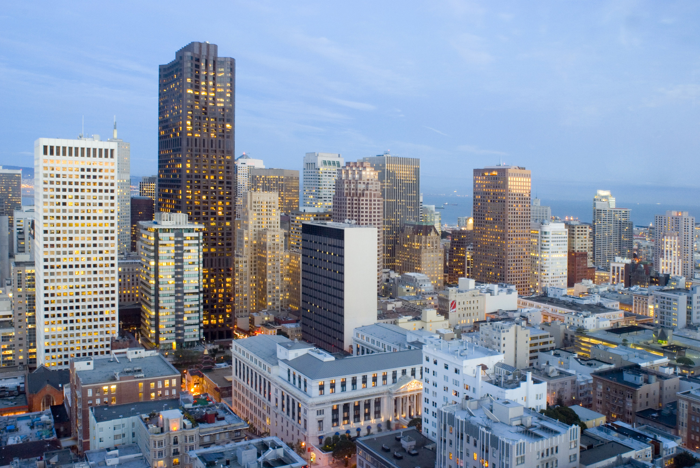
\includegraphics[height=5.2cm, width=1.01\textwidth]{d_content1}
        \label{fig:dpst_d_content1}
        \caption{Poza cu conținut}
	\end{subfigure}
    \hfill
    \begin{subfigure}[b]{0.49\textwidth}
		\centering
        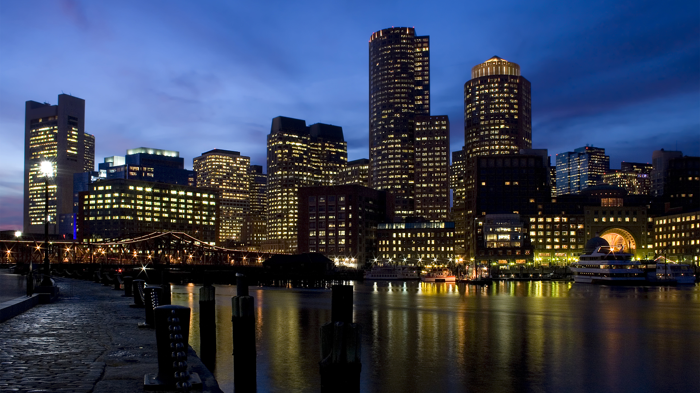
\includegraphics[height=5.2cm, width=1.01\textwidth]{d_style1}
        \label{fig:dpst_d_style1}
        \caption{Poza cu stil}
	\end{subfigure}
    \begin{subfigure}[b]{0.49\textwidth}
		\centering
        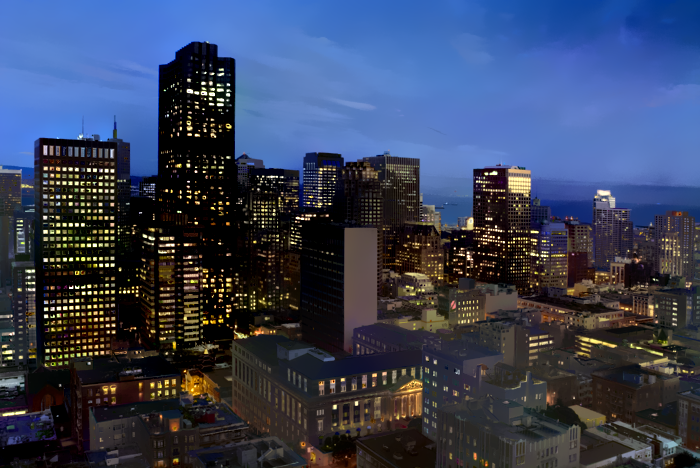
\includegraphics[height=5.2cm, width=1.01\textwidth]{dpst_c1s1_luan}
        \label{fig:dpst_c1s1_luan}
        \caption{Poză luată din articolul lui Fujun Luan}
	\end{subfigure}
    \hfill
    \begin{subfigure}[b]{0.49\textwidth}
		\centering
        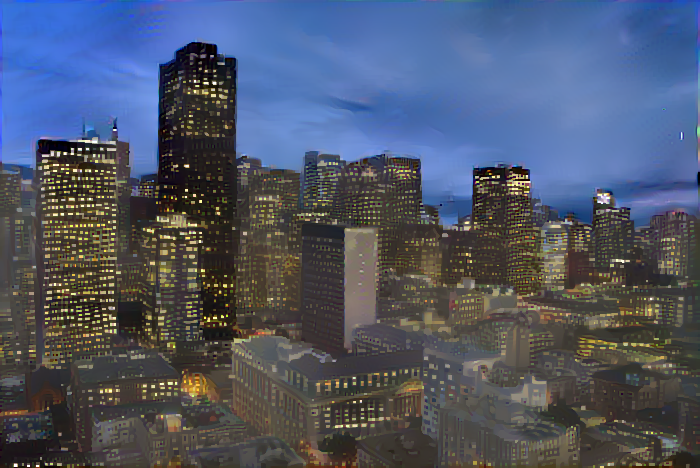
\includegraphics[height=5.2cm, width=1.01\textwidth]{dpst_c1s1}
        \label{fig:dpst_c1s1}
        \caption{Poză generată de mine}
	\end{subfigure}
    \caption{Cele două poze sunt diferite, deoarece în poza din stânga, autorul mai aplică unele optimizări în plus. De asemenea, mai intră în calcul și dimensiunea pozelor cu conținut și stil care au fost folosite la generarea celei de-a treia poze.}
\end{figure}

În continuare, voi mai prezenta și alte rezultate pentru a exemplifica posibilitățile pe care le oferă această metoda, cum ar fi schimbarea anotimpului dintr-o poză sau modificarea doar a anumitor obiecte din poză folosind măștile.

\begin{figure}[h]
	\centering
    \begin{subfigure}[b]{0.3\textwidth}
		\centering
        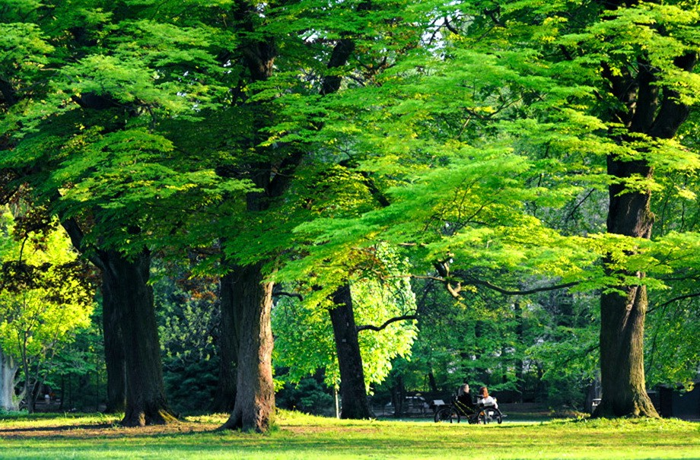
\includegraphics[height=4.7cm, width=1.01\textwidth]{d_content2}
        \label{fig:dpst_d_content2}
	\end{subfigure}
    \hfill
    \begin{subfigure}[b]{0.3\textwidth}
		\centering
        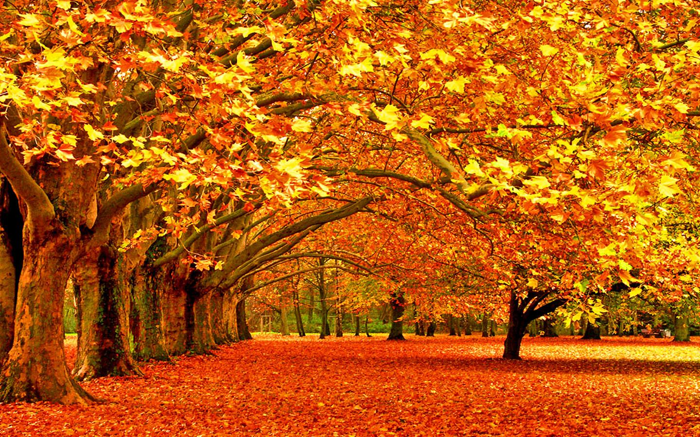
\includegraphics[height=4.7cm, width=1.01\textwidth]{d_style2}
        \label{fig:dpst_d_style2}
	\end{subfigure}
    \hfill
    \begin{subfigure}[b]{0.3\textwidth}
		\centering
        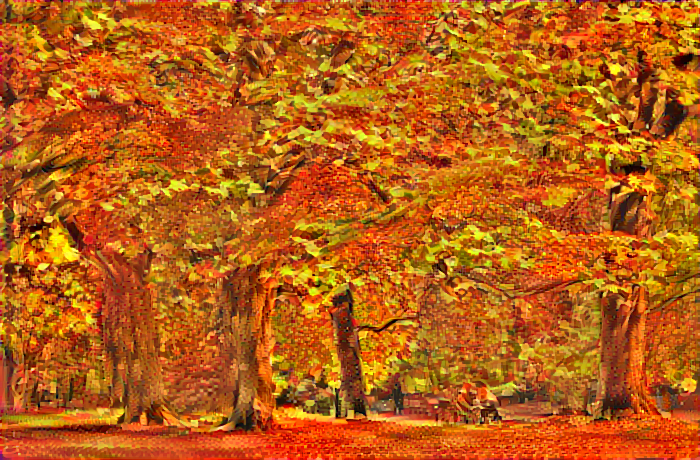
\includegraphics[height=4.7cm, width=1.01\textwidth]{dpst_c2s2}
        \label{fig:dpst_c2s2}
	\end{subfigure}
    \begin{subfigure}[b]{0.3\textwidth}
		\centering
        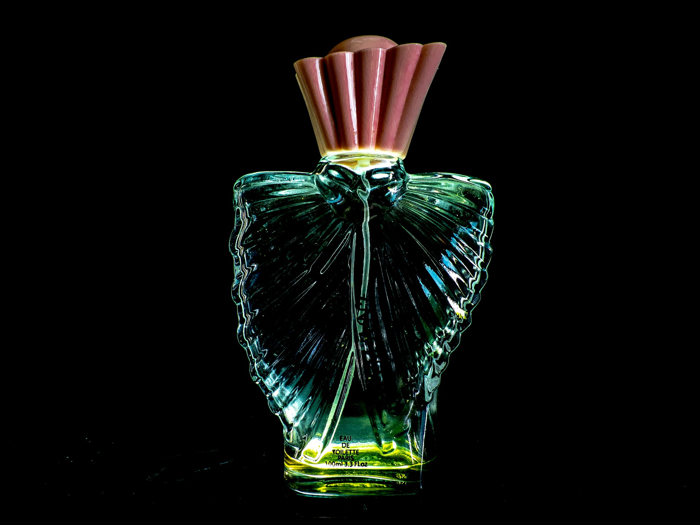
\includegraphics[height=4.7cm, width=1.01\textwidth]{d_content5}
        \label{fig:dpst_d_content5}
	\end{subfigure}
    \hfill
    \begin{subfigure}[b]{0.3\textwidth}
		\centering
        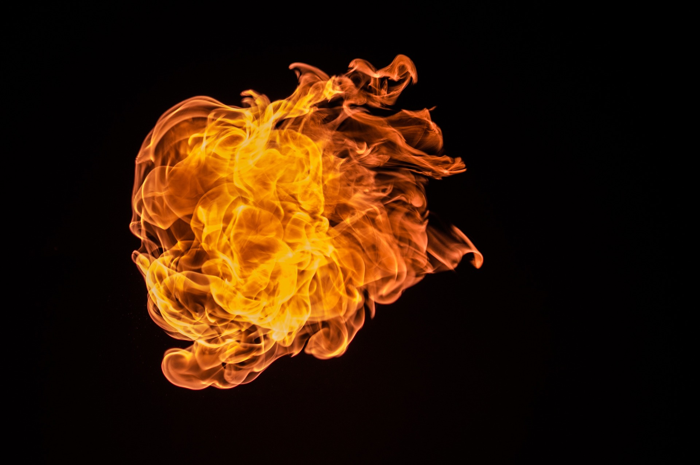
\includegraphics[height=4.7cm, width=1.01\textwidth]{d_style5}
        \label{fig:dpst_d_style5}
	\end{subfigure}
    \hfill
    \begin{subfigure}[b]{0.3\textwidth}
		\centering
        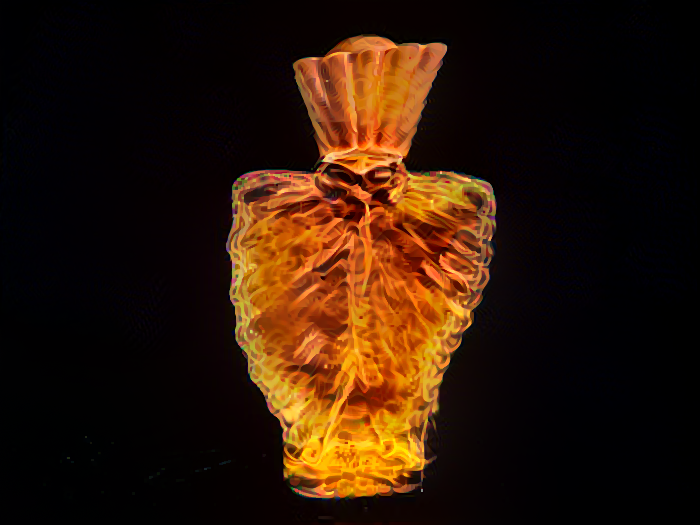
\includegraphics[height=4.7cm, width=1.01\textwidth]{dpst_c5s5}
        \label{fig:dpst_c5s5}
	\end{subfigure}
    \caption{}
\end{figure}

\begin{figure}[h]
	\centering
    \begin{subfigure}[b]{0.3\textwidth}
		\centering
        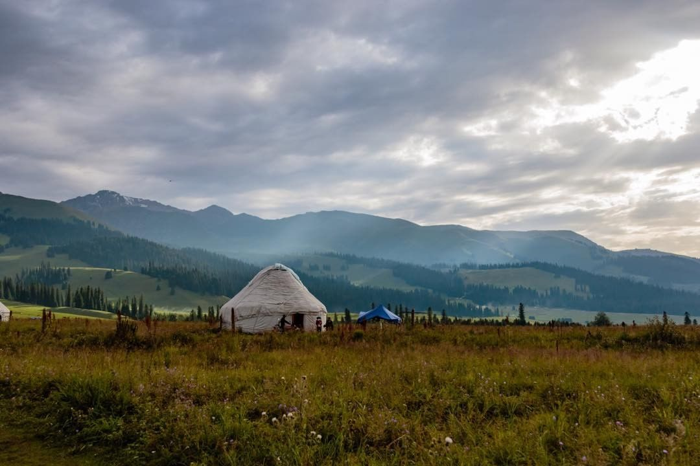
\includegraphics[height=4.7cm, width=1.01\textwidth]{d_content4}
        \label{fig:dpst_d_content4}
	\end{subfigure}
    \hfill
    \begin{subfigure}[b]{0.3\textwidth}
		\centering
        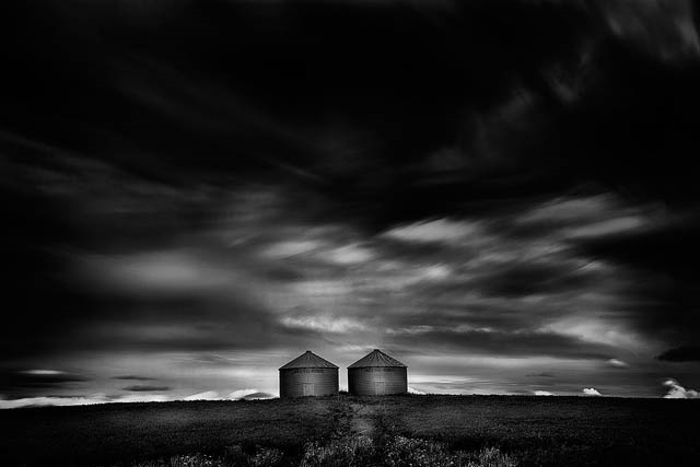
\includegraphics[height=4.7cm, width=1.01\textwidth]{d_style4}
        \label{fig:dpst_d_style4}
	\end{subfigure}
    \hfill
    \begin{subfigure}[b]{0.3\textwidth}
		\centering
        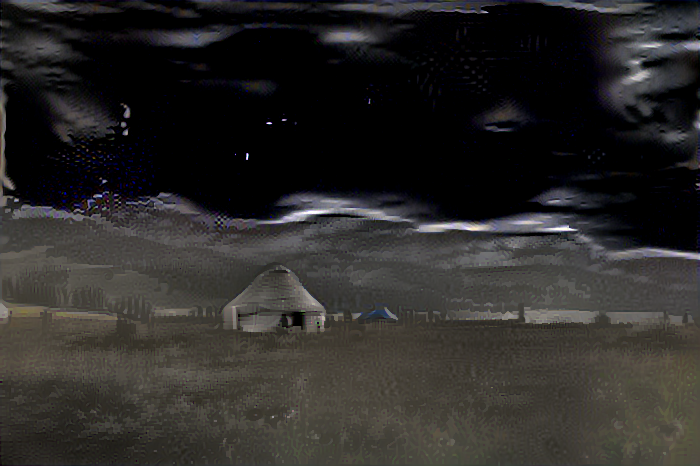
\includegraphics[height=4.7cm, width=1.01\textwidth]{dpst_c4s4}
        \label{fig:dpst_c4s4}
	\end{subfigure}
    \begin{subfigure}[b]{0.3\textwidth}
		\centering
        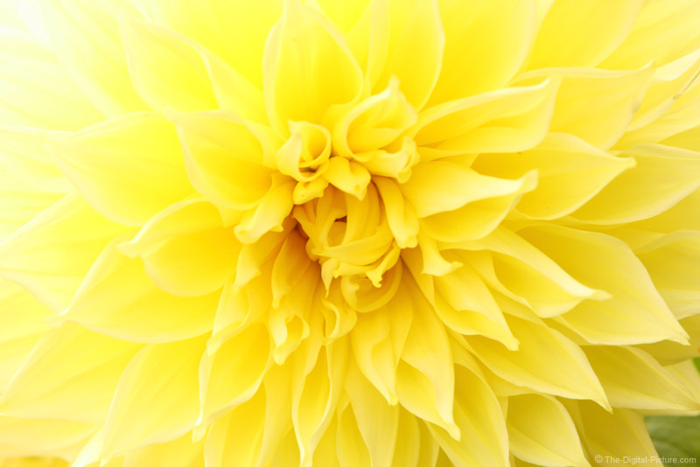
\includegraphics[height=4.7cm, width=1.01\textwidth]{d_content7}
        \label{fig:dpst_d_content7}
	\end{subfigure}
    \hfill
    \begin{subfigure}[b]{0.3\textwidth}
		\centering
        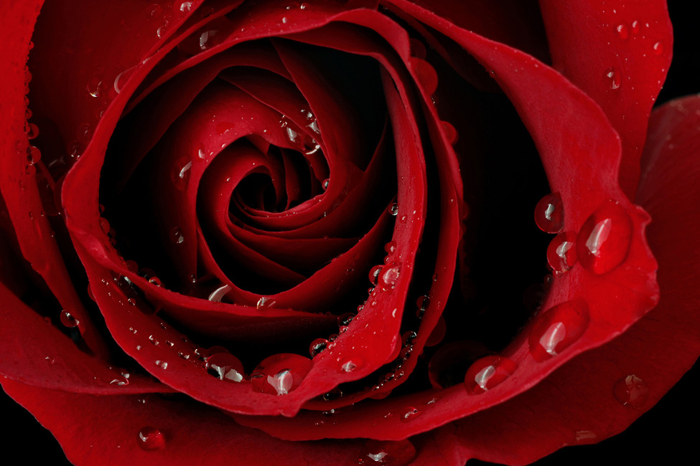
\includegraphics[height=4.7cm, width=1.01\textwidth]{d_style7}
        \label{fig:dpst_d_style7}
	\end{subfigure}
    \hfill
    \begin{subfigure}[b]{0.3\textwidth}
		\centering
        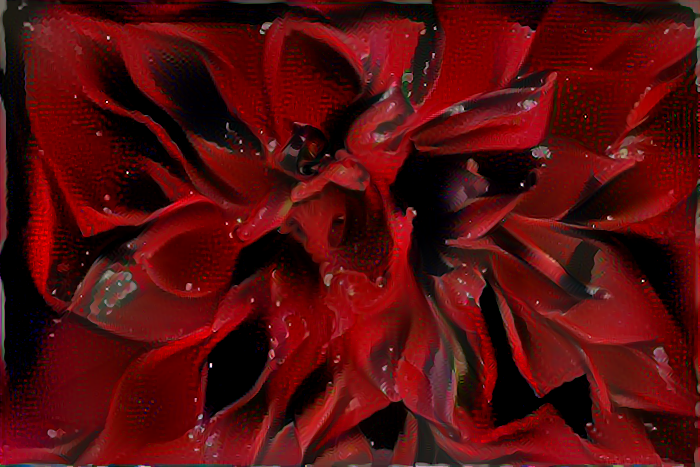
\includegraphics[height=4.7cm, width=1.01\textwidth]{dpst_c7s7}
        \label{fig:dpst_c7s7}
	\end{subfigure}
    \caption{Poze mai puțin reușite din cauza complexității și din cauza nepotrivirii intocmai a conținutului cu stilul.}
\end{figure}

\begin{figure}[h]
	\centering
    \begin{subfigure}[b]{0.24\textwidth}
		\centering
        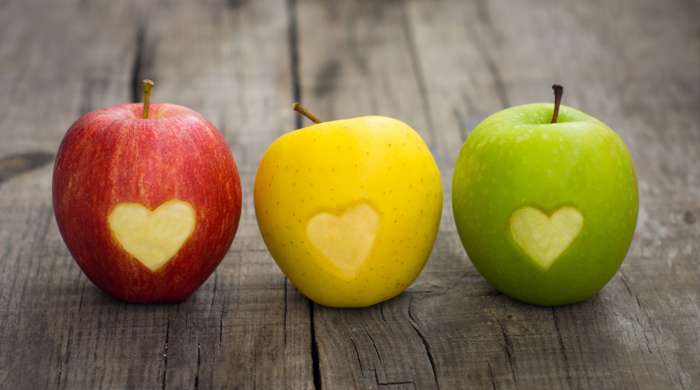
\includegraphics[height=3.5cm, width=1.01\textwidth]{d_content6}
        \label{fig:dpst_d_content6}
	\end{subfigure}
    \hfill
    \begin{subfigure}[b]{0.24\textwidth}
		\centering
        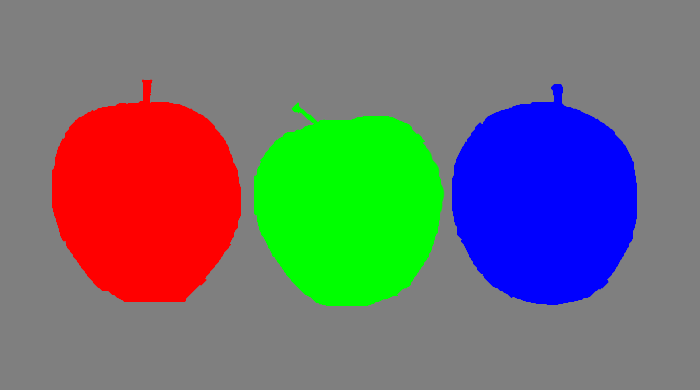
\includegraphics[height=3.5cm, width=1.01\textwidth]{mask_d_content6}
        \label{fig:dpst_d_mask_content6}
	\end{subfigure}
    \hfill
    \begin{subfigure}[b]{0.24\textwidth}
		\centering
        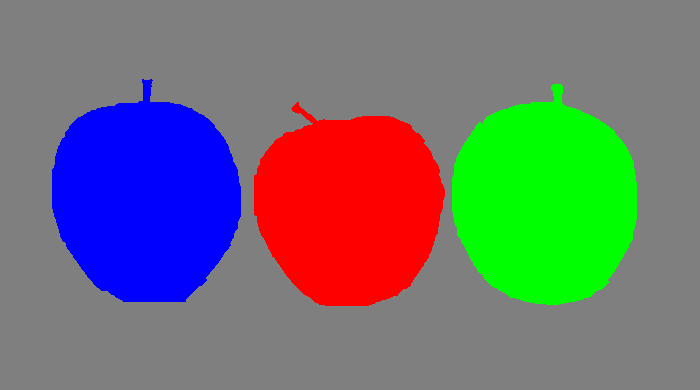
\includegraphics[height=3.5cm, width=1.01\textwidth]{mask_d_style6}
        \label{fig:dpst_d_mask_style6}
	\end{subfigure}
    \hfill
    \begin{subfigure}[b]{0.24\textwidth}
		\centering
        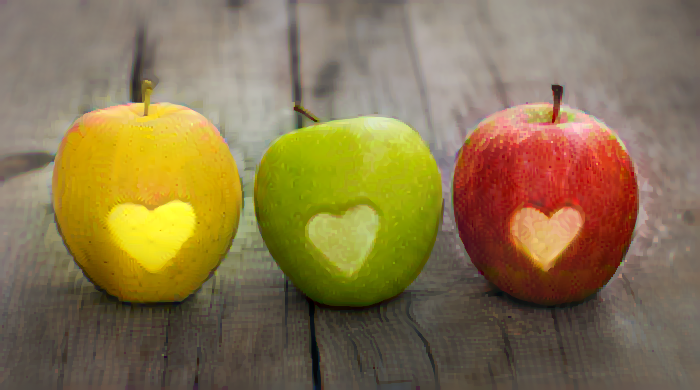
\includegraphics[height=3.5cm, width=1.01\textwidth]{dpst_c6s6}
        \label{fig:dpst_c6s6}
	\end{subfigure}
    \caption{În această figură se poate vedea avantajul măștii. Poza din stânga este tratată și ca poză de conținut și ca poză de stil. Poza a doua reprezintă masca pentru poza care este generată, iar a treia poză reprezintă masca pentru poza cu stil. Ultima poză este poza generată de către algoritm.}
\end{figure}

\begin{figure}[h]
	\centering
    \begin{subfigure}[b]{0.24\textwidth}
		\centering
        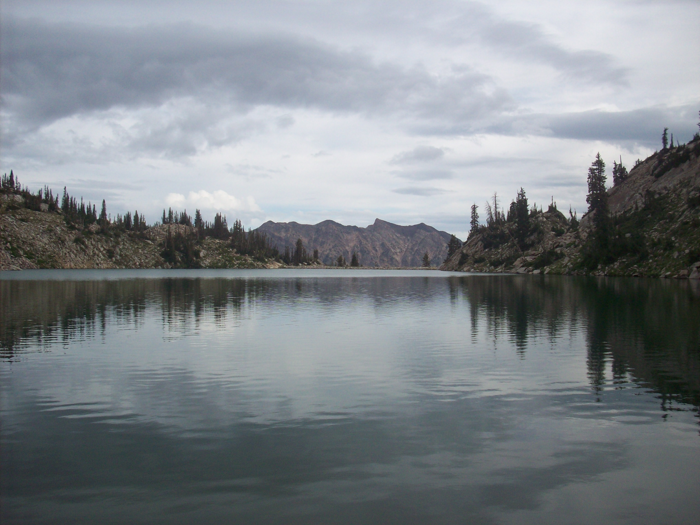
\includegraphics[height=4cm, width=1.01\textwidth]{d_content3}
        \label{fig:dpst_d_content3}
	\end{subfigure}
    \hfill
    \begin{subfigure}[b]{0.24\textwidth}
		\centering
        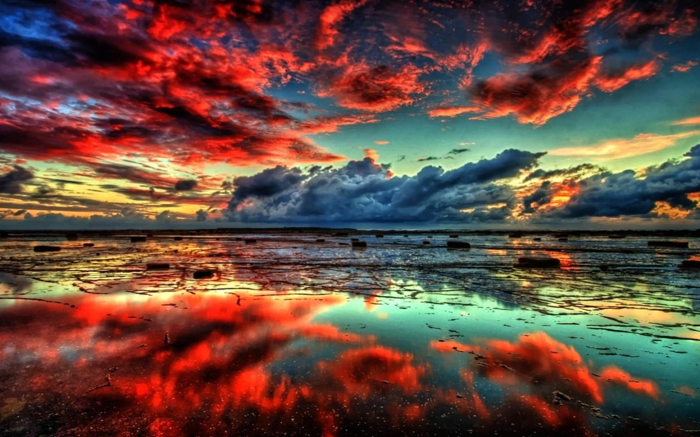
\includegraphics[height=4cm, width=1.01\textwidth]{d_style3}
        \label{fig:dpst_d_style3}
	\end{subfigure}
    \hfill
    \begin{subfigure}[b]{0.24\textwidth}
		\centering
        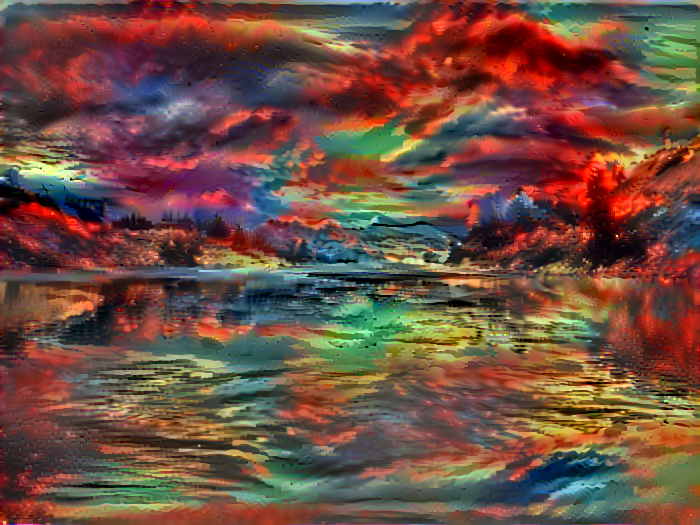
\includegraphics[height=4cm, width=1.01\textwidth]{dpst_c3s3}
        \label{fig:dpst_d_mask_style3}
	\end{subfigure}
    \hfill
    \begin{subfigure}[b]{0.24\textwidth}
		\centering
        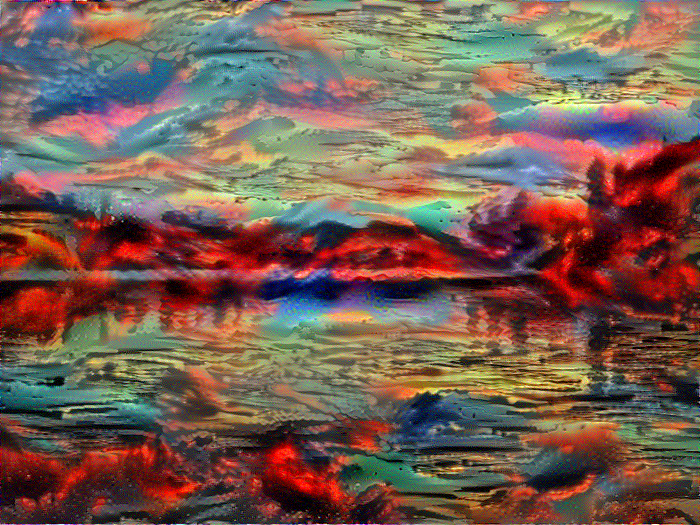
\includegraphics[height=4cm, width=1.01\textwidth]{dpst_c3s3_content}
        \label{fig:dpst_c3s3_content}
	\end{subfigure}
    \caption{În această figură, pentru generarea pozei a treia am pornit de la o poză inițializată cu zgomot, iar pentru generarea ultimei poze, am pornit de la o poză inițializată cu poza de conținut peste care am adăugat zgomot aleator. Se poate observa că folosind ultima metodă algoritmul învață mai ușor reprezentarea conținutului, iar stilul are un impact mai scăzut.}
\end{figure}

\begin{figure}[h]
	\centering
    \begin{subfigure}[b]{0.24\textwidth}
		\centering
        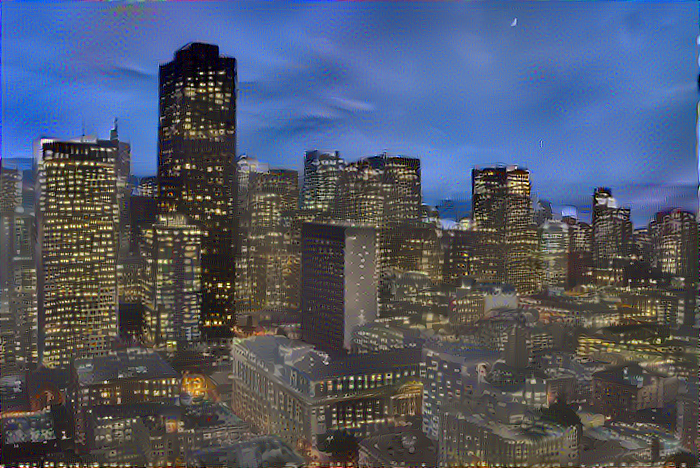
\includegraphics[height=4cm, width=1.01\textwidth]{dpst_c1s1_lambda0_001}
        \label{fig:dpst_c1s1_lambda0_001}
        \caption{$\gamma = 0.001$}
	\end{subfigure}
    \hfill
    \begin{subfigure}[b]{0.24\textwidth}
		\centering
        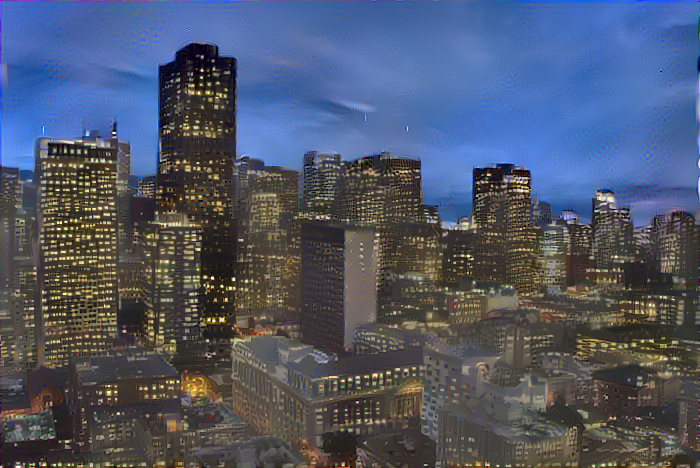
\includegraphics[height=4cm, width=1.01\textwidth]{dpst_c1s1_lambda0_01}
        \label{fig:dpst_c1s1_lambda0_01}
        \caption{$\gamma = 0.01$}
	\end{subfigure}
    \hfill
    \begin{subfigure}[b]{0.24\textwidth}
		\centering
        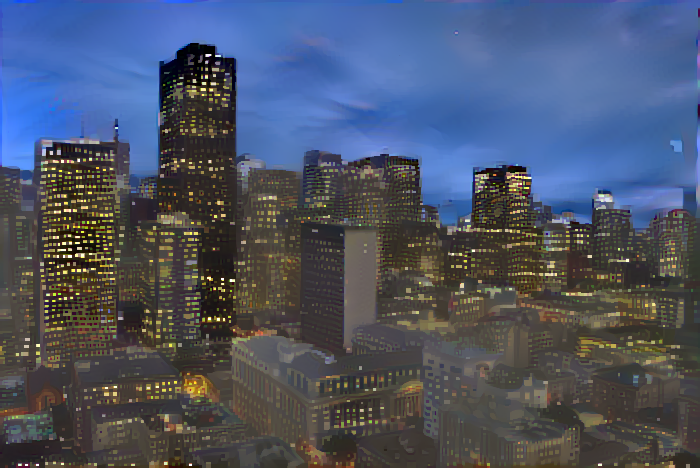
\includegraphics[height=4cm, width=1.01\textwidth]{dpst_c1s1_lambda0_1}
        \label{fig:dpst_c1s1_lambda0_1}
        \caption{$\gamma = 0.1$}
	\end{subfigure}
    \hfill
    \begin{subfigure}[b]{0.24\textwidth}
		\centering
        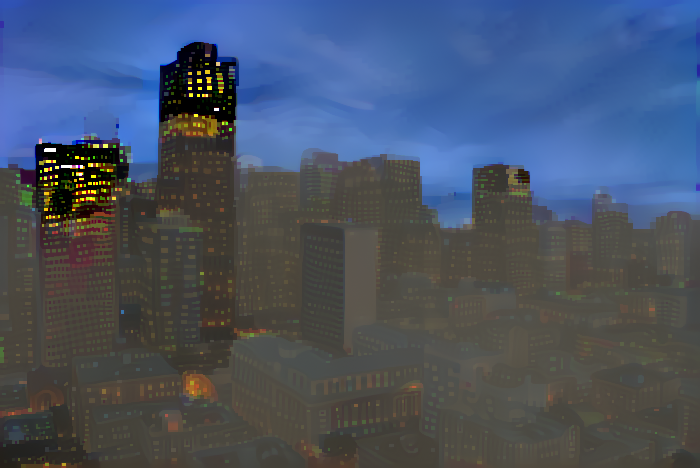
\includegraphics[height=4cm, width=1.01\textwidth]{dpst_c1s1_lambda1}
        \label{fig:dpst_c1s1_lambda1}
        \caption{$\gamma = 1$}
	\end{subfigure}
    \caption{În această figură se poate vedea impactul pe care îl are $\gamma$, parametrul care controlează importanța funcției de cost pentru zgomot.}
\end{figure}